
\subsection{Popis GUI} \label{popis-gui}
V této kapitole specifikujeme výstup STM tj. popíšeme co všechno a za jakých okolností
bude zobrazeno na displeji v daný moment.

% Stavy vzhledem ke GUI.
Nejprve specifikujeme v jakých stavech se STM může nacházet.
Toto jsou pouze stavy, které nás zajímavý v kontextu GUI - tj. v kontextu toho co všechno chceme
uživateli zobrazit.
Rozhodně se nejedná o souhrn všech možný stavů.
\subsubsection{Stavy STM}
\begin{itemize}
  \item Ethernetová periferie je korektně inicializována a kabel je připojen. Zkráceně budeme
        značit \texttt{ETH-up}.
  \item Ethernetový kabel je buď odpojen nebo ethernetová periferie se z nějakého důvodu
        neinicializovala. Zkráceně budeme značit jako \texttt{ETH-down}.
  \item STM je připojeno k serveru. Zkráceně značíme \texttt{CONNECTED}.
  \item STM je odpojeno od serveru. Zkráceně značíme \texttt{DISCONNECTED}.
  \item STM se připojuje k serveru. Zkráceně značíme \texttt{CONNECTING}.
  \item V EEPROM nejsou uložena žádná konfigurační data intervalů. Tento stav nastává pouze v případě,
        kdy uživatel zapne STM poprvé.
  \item V EEPROM jsou uložena konfigurační data intervalů.
  \item Uživatel už zadal klíč do STM. Tento klíč se ukládá do EEPROM, aby ho uživatel
        nemusel zadávat opakovaně.
  \item Uživatel ještě klíč nezadal. To znamená, že se ještě nepokoušel připojit k serveru.
\end{itemize}

% Invarianty - co chceme aby v rámci GUI platilo.
\subsubsection{Invarianty}
\begin{itemize}
  \item Odpojení resp. zapojení ethernetového kabelu když je STM zapnuté by nemělo způsobit žádnou chybu, což
    znamená, že stavy \texttt{ETH-up} a \texttt{ETH-down} se mohou libovolně střídat.
  \item Pokud se STM dostane do stavu \texttt{ETH-up}, dá uživateli možnost připojit se k serveru.
  \item Pokud je STM ve stavu \texttt{CONNECTED}, nemůže se od serveru odpojit.
    Jediná možnost jak STM odpojit od serveru je buď ho resetovat nebo odpojit ethernetový kabel.
  \item Pokud STM vůbec není připojeno k internetu a EEPROM je prázdná, umožní STM uživateli nastavit
    intervaly.
\end{itemize}

% Popis jednotlivých obrazovek
\subsubsection{Popis jednotlivých obrazovek}

% Vyjmenování GUI prvků, které budeme potřebovat
V rámci celého GUI nám stačí tyto grafické prvky:
\begin{itemize}
  \item Tlačítka, pomocí kterých uživatel buď potvrdí zadaná data, nebo je zahodí.
    Kromě toho tlačítka ještě umožňují přepínání mezi jednotlivými obrazovkami.
  \item Okna s nastavitelnou hodnotou kde hodnota může být například čas v minutách, nebo teplota.
    Uživatel může hodnotu nastavit pomocí joysticku.
  \item Okna, která slouží pouze pro zobrazování nějaké hodnoty - například aktuálního času, nebo
    naměřené teploty.
  \item Různé nápisy resp. nadpisy pro lepší přehlednost.
\end{itemize}

Nejprve uvedeme nákresy jednotlivých obrazovek a popíšeme co znamenají.
Potom uvedeme tzv. frame diagram tj. stavový diagram obrazovek, kde popíšeme jak se mezi sebou
jednotlivé obrazovky přepínají.
Zeleně zabarvený text v obrázcích představuje buď nakliknutelný čudlík nebo měnitelný prvek - například čas.
Jak jsme již zmiňovali STM se ovládá pomocí joysticku pod displejem.
Pohybem joysticku do stran přepínáme mezi jednotlivými nakliknutelnými prvky.
Pohybem joysticku nahoru a dolu měníme hodnoty právě nakliknutých prvků, pokud to jde.
Nakliknutý prvek na displeji STM poznáme podle červeného zabarvení.

Jednotlivé obrazovky jsou pojmenovány podle názvů tříd (v C++), které je reprezentují a jsou zmíněny
v kapitole architektura.

% ClkFrame
\paragraph{ClkFrame}
\begin{figure}[H]\centering
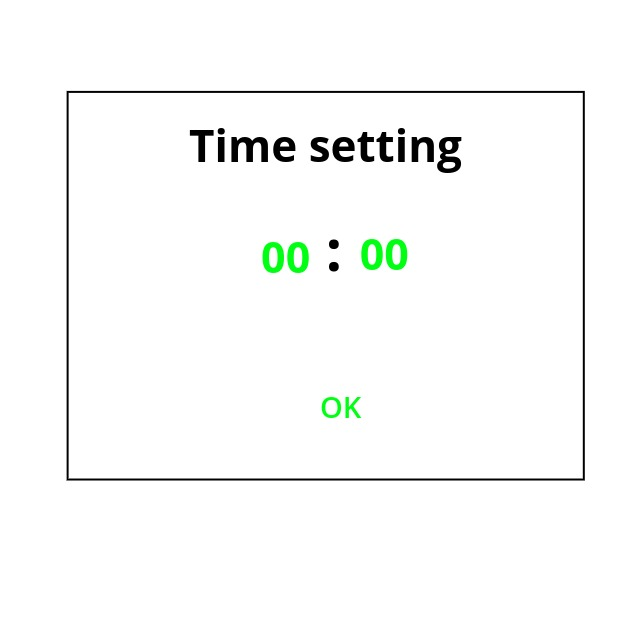
\includegraphics[width=100mm, height=100mm]{../img/clk_frame.jpg}
\caption{ClkFrame - nastavení času}
\label{clk-frame}
\end{figure}

Obrazovka \ref{clk-frame} je zobrazena po startu STM v momentě, kdy ethernetová periferie není inicializována a
STM se tedy nemůže připojit k serveru aby mohlo rovnou synchronizovat čas se serverem.
Uživatel musí nastavit nějaký čas (není nutné aby odpovídal reálnému času), aby STM vědělo, který
interval je aktuální a tedy jakou teplotu má udržovat.

% SetIntervalFrame
\paragraph{SetIntervalFrame}
\begin{figure}[H]\centering
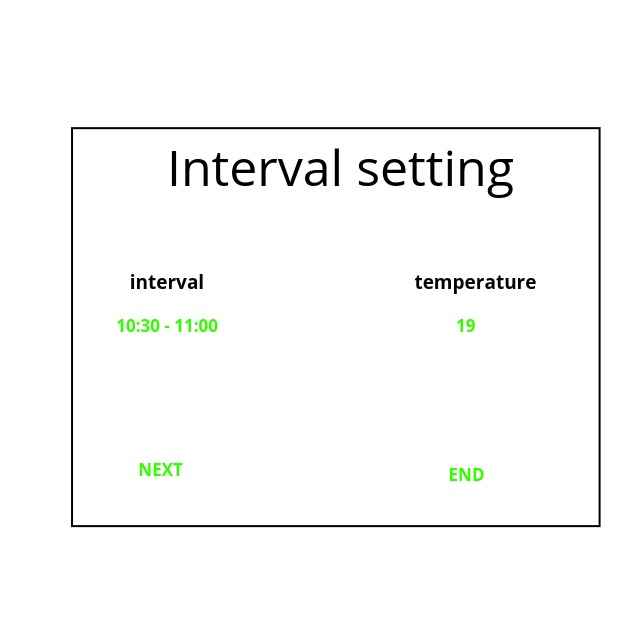
\includegraphics[width=100mm, height=100mm]{../img/interval_setting_frame.jpg}
\caption{SetIntervalFrame - nastavení intervalů}
\label{set-interval-frame}
\end{figure}

Obrazovka \ref{set-interval-frame} umožňuje uživateli nastavit časové intervaly s teplotou.
Obrazovka zobrazuje nastavení pro právě jeden interval, pokud uživatel stiskne tlačítko
\uv{Next}, zobrazí se nastavení dalšího intervalu, pokud stiskne tlačítko \uv{End}, nastavování
intervalů se ukončí a všechny nastavené intervaly jsou uloženy do EEPROM.

Zobrazena je v těchto případech:
\begin{itemize}
  \item když EEPROM neobsahuje žádné nastavení intervalů což nastává v případě kdy uživatel
    ještě žádné intervaly nenastavoval - tedy po prvním spuštění STM.
  \item Když uživatel zmáčkne v obrazovce \texttt{MainFrame} tlačítko \uv{reset intervals}.
\end{itemize}

% OverviewIntervalFrame
\paragraph{OverviewIntervalFrame}
\texttt{OverviewIntervalFrame} neboli \uv{přehled všech nastavených intervalů} vypadá stejně
jako \texttt{SetIntervalFrame} až na to, že intervaly nejdou nastavovat, pouze prohlížet.
Tlačítkem \uv{Next} se uživatel prokliká postupně přes všechny intervaly a tlačítkem \uv{End} zobrazování
ukončí.

% ConnectFrame
\paragraph{ConnectFrame}
\begin{figure}[H]\centering
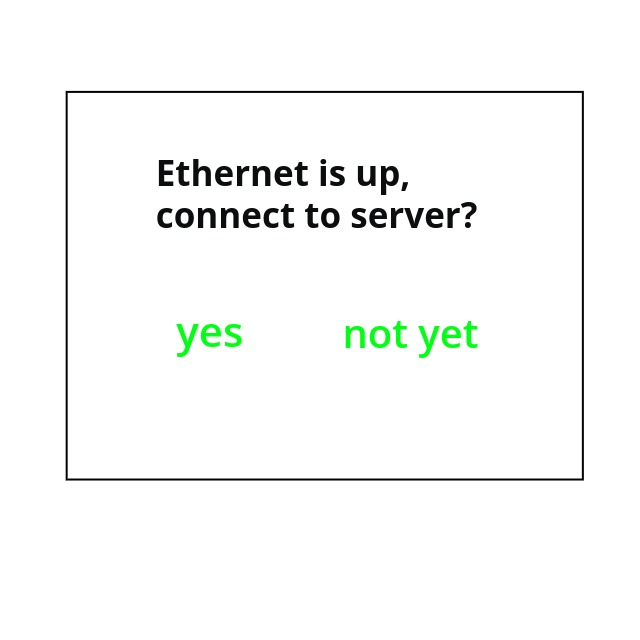
\includegraphics[width=100mm, height=100mm]{../img/connect_frame.jpg}
\caption{ConnectFrame - připojení k serveru}
\label{connect-frame}
\end{figure}

Obrazovka \ref{connect-frame} je zobrazena ihned po spuštění STM v momentě, kdy ethernetová periferie je inicializována
a klíč ještě není uložen v EEPROM.
V takovém případě se STM může ihned připojit k serveru a nemusíme uživatele zdržovat s nastavováním
času.

% KeyFrame
\paragraph{KeyFrame}
\begin{figure}[H]\centering
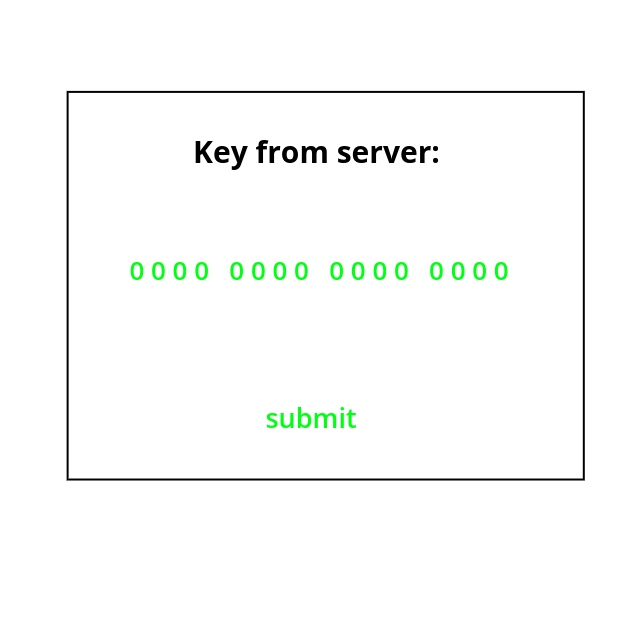
\includegraphics[width=100mm, height=100mm]{../img/key_frame.jpg}
\caption{KeyFrame - zadání klíče vygenerovaného serverem}
\label{key-frame}
\end{figure}

Do obrazovky \ref{key-frame} uživatel zadá osmi bajtový DES klíč \cite{DES} vygenerovaný na serveru.
Po stisknutí tlačítka \uv{Submit} se STM pokusí přihlásit na server.

% MainFrame
\paragraph{MainFrame}
\begin{figure}[H]\centering
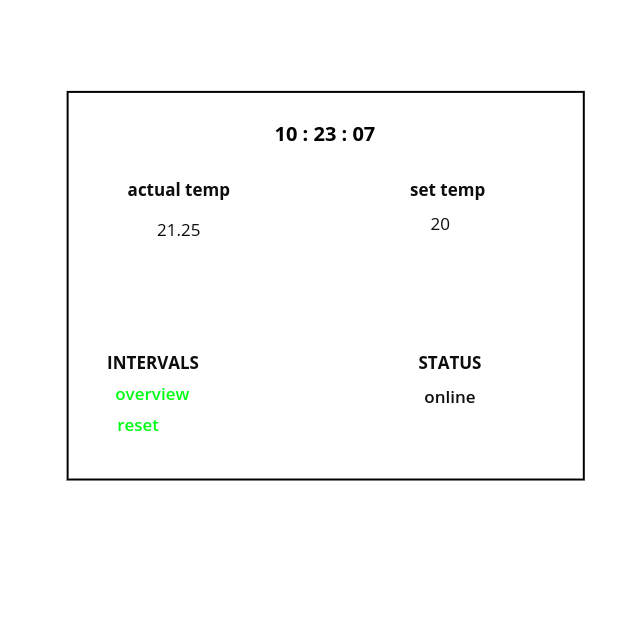
\includegraphics[width=100mm, height=100mm]{../img/main_frame_online.jpg}
\caption{MainFrame - hlavní obrazovka}
\label{main-frame}
\end{figure}

MainFrame (\ref{main-frame}) reprezentuje hlavní obrazovku.
Jsou zde zobrazeny zásadní hodnoty - aktuálně naměřená teplota (actual temp), přednastavená teplota
(set temp) a stav připojení k serveru.
% tlačítko connect
Pokud je STM ve stavu \texttt{DISCONNECTED} a zároveň \texttt{ETH-up}, zobrazí v \texttt{MainFrame}
tlačítko \uv{connect}, pomocí kterého se uživatel dostane na obrazovku \texttt{KeyFrame}, do které zadá klíč
vygenerovaný serverem a připojí se tak k serveru.
V případě kdy je klíč uložen v EEPROM, tak se STM po stisku tlačítka \uv{connect} rovnou připojí k serveru
a pouze zobrazí stav \texttt{CONNECTING}.

Uživatel se z \texttt{MainFrame} také může dostat do \texttt{SetIntervalFrame} pomocí \uv{reset intervals}
tlačítka a do \texttt{OverviewIntervalFrame} pomocí \uv{overview intervals} tlačítka.

%%%%%%%%%%%%%%%
% Frame diagram
%%%%%%%%%%%%%%%
\subsubsection{Vztahy mezi obrazovkami}

\begin{figure}[tbh!]
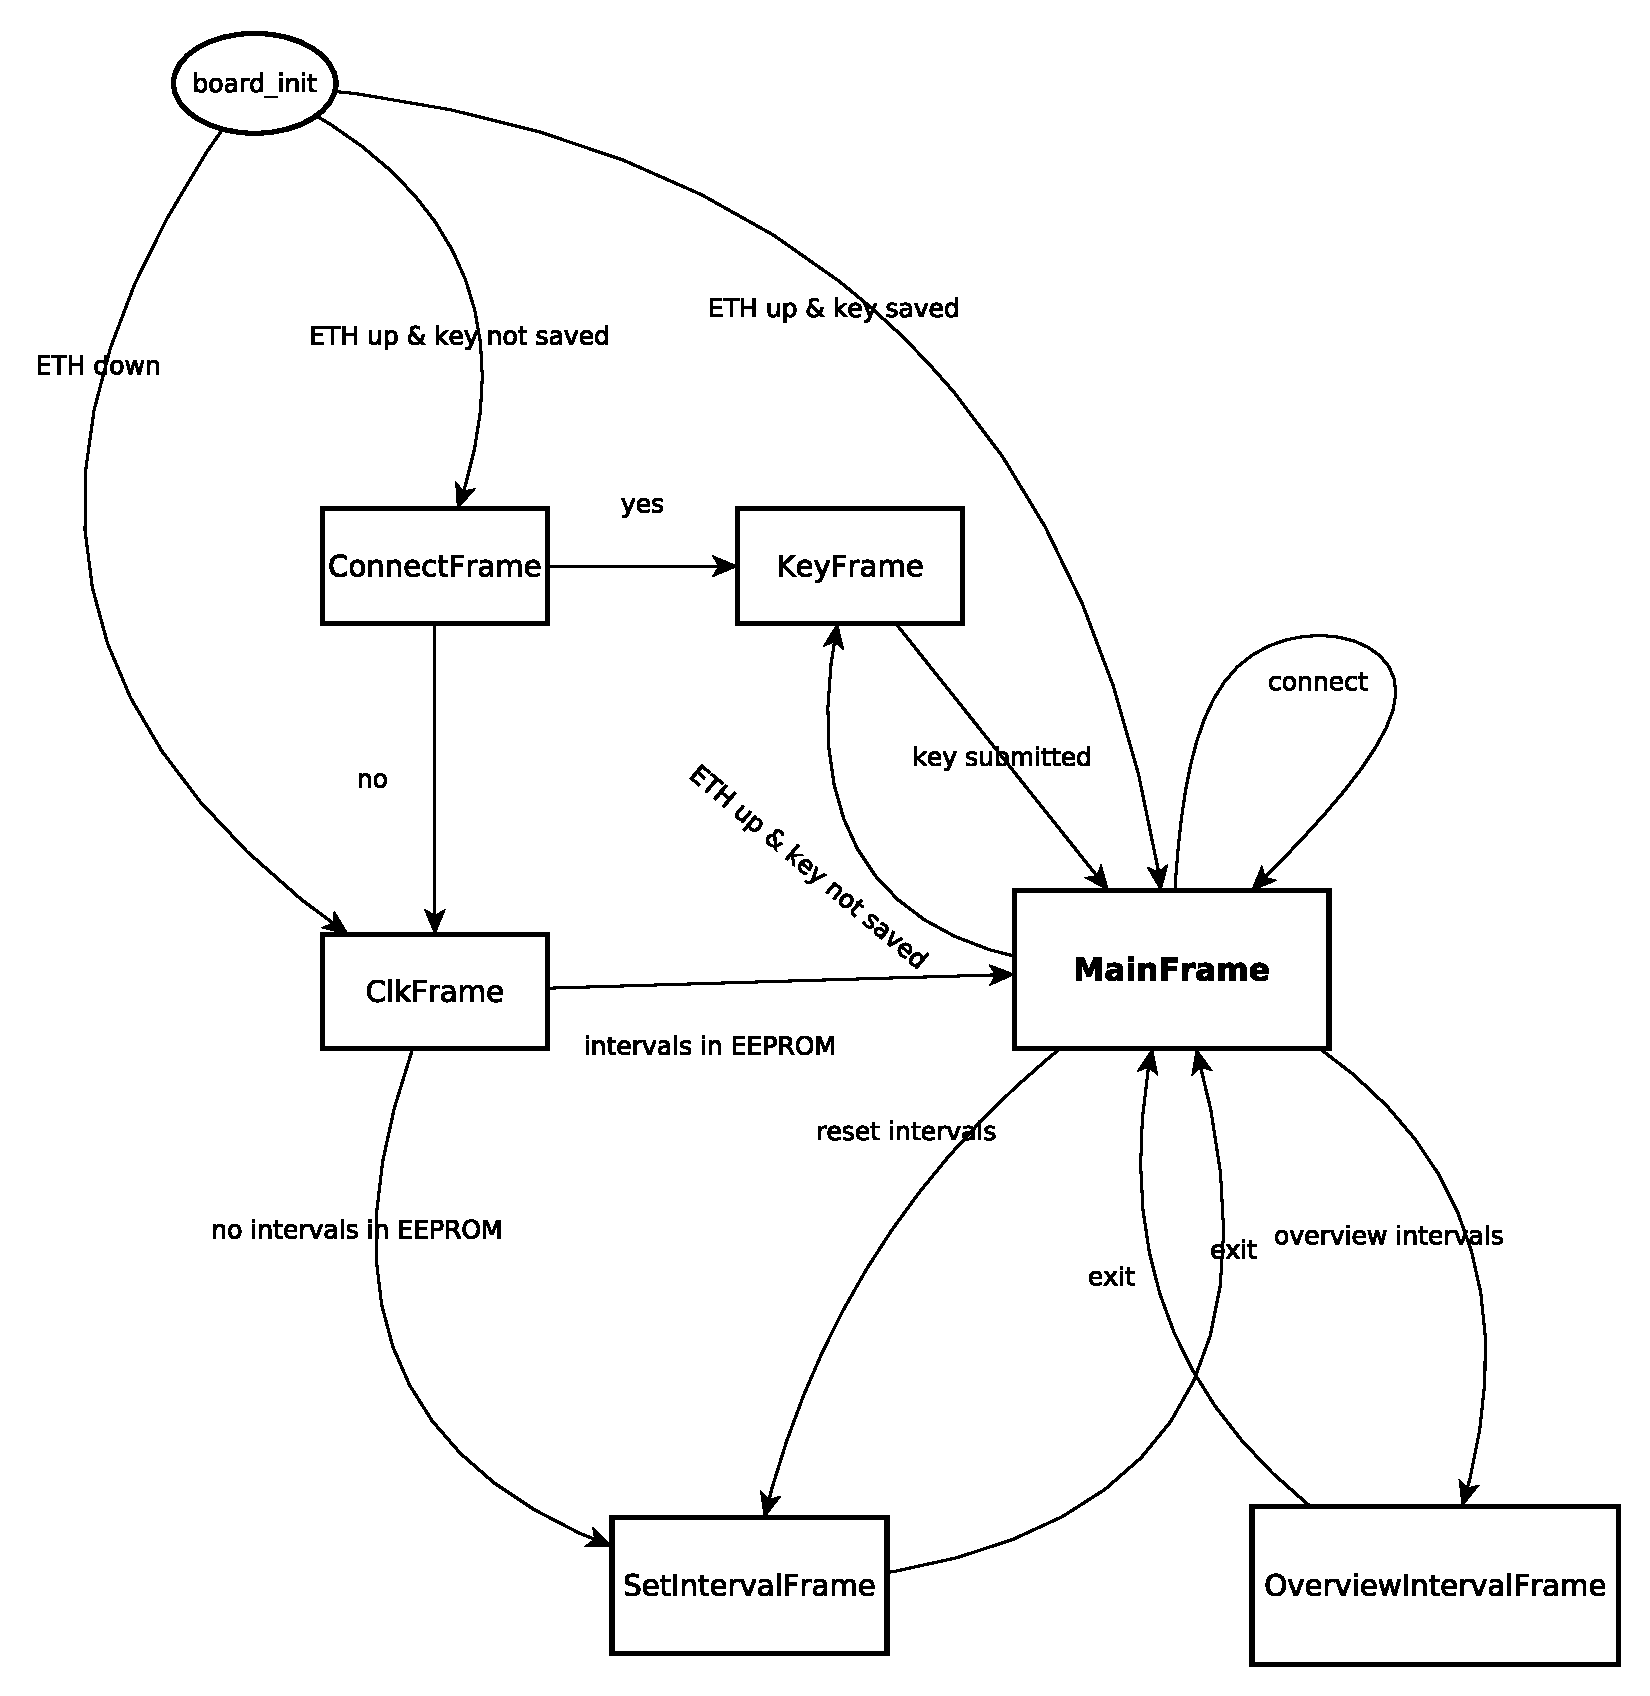
\includegraphics[scale=0.51]{../diagrams/frame_diagram.pdf}
\caption{Diagram přepínání obrazovek}
\label{frame-diagram}
\end{figure}

Diagram \ref{frame-diagram} je v podstatě orientovaný graf s počátečním uzlem \texttt{board\_init}
a koncovým uzlem \texttt{MainFrame}.
\texttt{ClkFrame} a \texttt{SetIntervalFrame} představují konfigurační obrazovky, které se postupně
zobrazí v případě kdy je STM offline nebo je spuštěno poprvé.
Po zadání konfigurace, je-li to nutné, se uživatel nakonec dostane do \texttt{MainFrame}, ze kterého
už může prohlížet jednotlivé intervaly v \texttt{OverviewIntervalFrame}, případně všechny intervaly
přenastavit v \texttt{SetIntervalFrame}.
Dále se z \texttt{MainFrame} může uživatel ještě dostat do \texttt{KeyFrame}, pokud se chce připojit
k serveru a klíč ještě není uložen v EEPROM.

